\subsection{Glyph: \glyph{Multimer}}
\label{sec:multimer}

As its name implies, a multimer is an aggregation of multiple identical or pseudo-identical entities held together by non-covalent bonds (thus, they are distinguished from polymers by the fact that the later involve covalent bonds).
Here,  \emph{pseudo-identical} refers to the possibility that the entities differ chemically but retain some common global characteristic, such as a structure or function, and so can be considered identical within the context of the SBGN \PD.
An example of this is the homologous subunits in a hetero-oligomeric receptor.

SBGN \PD defines four different \glyph{multimer} glyphs: \glyph{simple chemical multimer}, \glyph{macromolecule multimer}, \glyph{nucleic acid feature multimer} and \glyph{complex multimer}.



\begin{glyphDescription}

\glyphSboTerm
\begin{tabular}{l l}
    & SBO:0000286 ! multimer\\
\glyph{Simple chemical multimer} & SBO:0000421 ! multimer of simple chemicals\\
\glyph{Macromolecule multimer} & SBO:0000420 ! multimer of macromolecules \\
\glyph{Complex multimer} & SBO:0000418 ! multimer of complexes \\
\glyph{Nucleic acid feature multimer} & SBO:0000419 ! multimer of informational molecule segments \\
\end{tabular}


\glyphIncoming
Zero or more \glyph{production} arcs (\sect{production}).



\glyphOutgoing
Zero or more \glyph{consumption} arcs (\sect{consumption}), \glyph{modulation arcs} (\sect{modulations}), \glyph{logic arcs} (\sect{logicArc}), or \glyph{equivalence arcs} (\sect{equivalenceArc}).



\glyphContainer
Each \glyph{multimer} is represented by a different shape depending on the bio-molecular nature of its pseudo-identical subunits, as shown in \tab{multimer_containers}.
The shape of a \glyph{multimer} consists of two \glyph{subunits} or \glyph{EPNs} shapes shifted horizontally and vertically, and stacked on top of another.




\glyphLabel
A \glyph{subunit} is identified by a label that is   a string of characters that may be distributed on several lines to improve readability.
% 
The centre of the label must be placed on the centre of the shape.
The label may extend outside of the shape.
The label should refer to the pseudo-identical subunits, and not to the multimer itself.



\glyphAux A \glyph{multimer} may carry auxiliary units, depending on its type.

A \glyph{macromolecule}, \glyph{nucleic acid feature}, or \glyph{complex multimer} can carry one or more \glyph{state variables} that add information about its state (\sect{stateVariable}).
The state of such a \glyph{multimer} is defined as the set of all its \glyph{state variables}.

A \glyph{multimer} of any type can carry one or more \glyph{units of information} (\sect{unitInfo}).
These can characterize a domain, such as a binding site.
Particular \glyph{units of information} are available for describing the material type (\sect{material-types-cv}), conceptual type (\sect{conceptual-types-cv}) and the cardinality (\sect{cardinality-cv}) of such a \glyph{multimer}.

Note that a \glyph{state variable} or a \glyph{unit of information} carried by a \glyph{multimer} actually applies to each of the subunits individually.
If instead the \glyph{state variables} or the \glyph{units of information} are meant to apply to the whole multimeric assembly, a \glyph{macromolecule} (\sect{macromolecule}) or a \glyph{complex} (\sect{complex}) should be used instead of a \glyph{multimer}.
An assembly containing some \glyph{state variables} or \glyph{units of information} applicable to the subunits, and other \glyph{state variables} or \glyph{units of information} applicable to the assembly (for instance opening of a channel and phosphorylation of each of its subunits) should be represented by a \glyph{complex} (\sect{complex}).

Finally, a \glyph{simple chemical multimer} can also carry a \glyph{simple clone marker} (\sect{cloneMarker}), and a \glyph{macromolecule}, \glyph{nucleic acid feature} or \glyph{complex multimer} a \glyph{labelled clone marker} (\sect{cloneMarker}).

\end{glyphDescription}

\begin{table}[h]
\begin{tabu}{X[c,m]X[c,m]X[c,m]X[c,m]}
    \toprule
    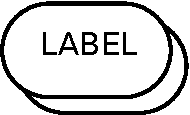
\includegraphics[valign=m]{images/build/simple_chemical_multimer.pdf} & 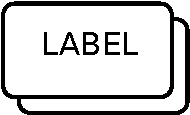
\includegraphics[valign=m]{images/build/macromolecule_multimer.pdf} & 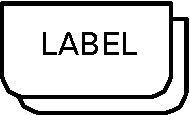
\includegraphics[valign=m]{images/build/genetic_multimer.pdf} & 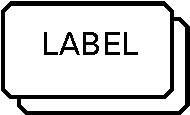
\includegraphics[valign=m]{images/build/complex_multimer.pdf}\\[0.5cm]
    \glyph{simple chemical multimer} & \glyph{macromolecule multimer} & \glyph{nucleic acid feature multimer} & \glyph{complex multimer}\\
	\bottomrule
\end{tabu}
\caption{The \PD glyphs for the different types of \glyph{multimers}.}
\label{tab:multimer_containers}
\end{table}

% \begin{figure}[H]
%   \centering
%   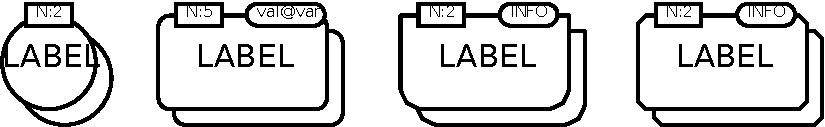
\includegraphics[scale=0.3]{images/build/multimer.pdf}
%   \caption{The \PD glyph for \glyph{multimer} with an additional unit of information containing the cardinality.}
%   \label{fig:multimer}
% \end{figure}
% 

% The following is for [X]Emacs users.  Please leave in place.
% Local Variables:
% TeX-master: "../sbgn_PD-level1"
% End:
